%\beginsupplement

\renewcommand{\thefigure}{A\arabic{figure}}
\setcounter{figure}{0}
\renewcommand{\thetable}{A\arabic{table}}
\setcounter{table}{0}

\section{Supplementary Data}
\label{supplinfo}


\subsection{Potentials}
isoPAHAP tables?
curPAHIP tables?

The atomic coordinates and charges of the minimised 2pent15ring monomer.
Probably should also include the same for corannulene (can pull from CST paper).

\subsection{Calculation of radial distances and coordination numbers}
\label{secSI:raddist_CN_eqns}
%
Average radial distances and coordination numbers are calculated to provide insight into molecular arrangements and cluster structure. The average radial distance of molecule type $k$, $r_{k}$, is calculated using the following equation:
\begin{equation}
    r_{k} = \frac{1}{N_{k}}\sum_{m \in I_{k}}R_{m}
\end{equation}
where $N_{k}$ is the number of molecules within $k \in \{\text{small},\text{large}\}$, referring to the small and large curved molecule types, $I_{k}$ is the set of molecule indices within $k$, and $R_{m}$ is the radial distance between the cluster geometric centre and the geometric centre of molecule $m$.

The coordination number of molecule type $k$, $CN_{k},$ provides the average number of molecules within a distance $R^{(\text{cutoff})}$. This is calculated as the average of the cumulative radial distribution function integrated over the centre of the cluster (set as the origin at 0) to a maximum cut-off radial distance, $R^{(\text{cutoff})}$:
\begin{equation}
    CN_{k}(R^{(\text{cut-off})}) = \frac{1}{N_{k}} \sum_{m \in I_{k}} \int\limits_{0}^{R^{(\text{cut-off})}}  \sum_{j=1}^{N_{\text{total}}} \delta(D_{mj} - R) dR
\end{equation}
$k \in \{\text{small}, \text{large}, \text{total}\}$ refers to the small curved molecules, large curved molecules, and all curved molecules within the cluster, respectively. $D_{mj}$ is the distance between the geometric centres of molecules $m$ and $j$. $R^{(\text{cut-off})}$ corresponds to the radius of the molecule type of interest, so $R^{(\text{cut-off})}_{\text{PYR}} = 0.46$ nm, $R^{(\text{cut-off})}_{\text{COR}} = 0.47$ nm, $R^{(\text{cut-off})}_{\text{OVA}} = 0.59$ nm, and $R^{(\text{cut-off})}_{\text{CIR}} = 0.71$ nm. $CN_{\text{total}}$ values use the radius of the larger molecule in the system considered. These provide $CN$ values from zero to two, corresponding to an isolated molecule and a molecule sandwiched between two others, respectively.

% rewrite above so that 'small' = corannulene, 'large' = 2pent15ring

%\subsection{Position restraint negligibility at low temperature}

\subsection{Simulation length equilibration check}
Energies and radial distances don't change significantly when comparing eqm result from 3ns simulation (final 1ns) or 1ns simulation (final 500ps)
Percent error of intermolecular energies are less than 0.2\%
Percent error of radial distances are less than 3.5\%



\subsection{Corannulene crystal structure}
In order to assess / benchmark the structural metrics used in this paper, they have been applied to the known crystal structure of a corannulene. %Further comparison is made with a 2pent15ring system and published large cPAH systems - Actually this should be included in the discussion sections of the paper I think.

X-ray analysis of corannulene was conducted in 1975, and it was determined that the compound crystallises in space group \textit{P}$2_{1}/c$ \cite{hanson1976crystal}.

A crystal structure containing 18 molecules, taken from The Cambridge Crystallographic Data Centre \cite{CORANN11unitcell}, provides an independent verification of the analysis used in this work as well as a known experimental structure useful for comparison.  The crystal density and intermolecular distances are provided in Table \ref{tableSI:crystal}.  Figure XX shows the crystal structure and alignment angles.

\begin{table}[]
\centering
\caption{Molecular configuration metrics of corannulene crystal structure (collected from \cite{CORANN11unitcell}).}
\label{table:crystal}
\begin{tabular}{cc|cll}
\multicolumn{2}{c}{Density (kg/m3)} & 1.36 \cite{CORANN11unitcell}&  &  \\ \cline{1-3}
\multirow{3}{*}{Average intermolecular distance (nm)} & 1 molecule & 0.57 &  &  \\
 & 2 molecule & 0.72 &  &  \\
 & 3 molecule & 0.76 &  &  \\ \cline{1-3}
\multirow{3}{*}{Intermolecular distances (nm)} & 1 molecule & 0.55 x 10, 0.61 x 6 &  &  \\
 & 2 molecules & 0.61 x 2, 0.72 x 10, 0.73 x 2, 0.76 x 2, 0.78 x 2 &  &  \\
 & 3 molecules & 0.72 x 2, 0.73 x 4, 0.76 x 8, 0.78 x 2, 0.82 x 2 &  & 
\end{tabular}
\end{table}
%
%(using cut-off value of $R = 0.7$ nm)
%Intermolecular distances: 0.55 nm x 10, 0.61 nm x 6 (for first molecule); 0.61 x 2, 0.72 x 10, 0.73 x 2, 0.76 x 2, 0.78 x 2 (for second molecule), 0.72 x 2, 0.73 x 4, 0.76 x 8, 0.78 x 2, 0.82 x 2 (third molecule)... NOT SURE HOW TO SHOW THESE -> FOLLOW SAME PATTERN USED IN HOW I DISCUSS THIS IN THE PAPER (AVERAGE INTERMOLECULAR DISTS? - WOULD BE 0.57 NM FOR FIRST MOLECULE, ETC)
%
\begin{figure}[!tbh]
\centering
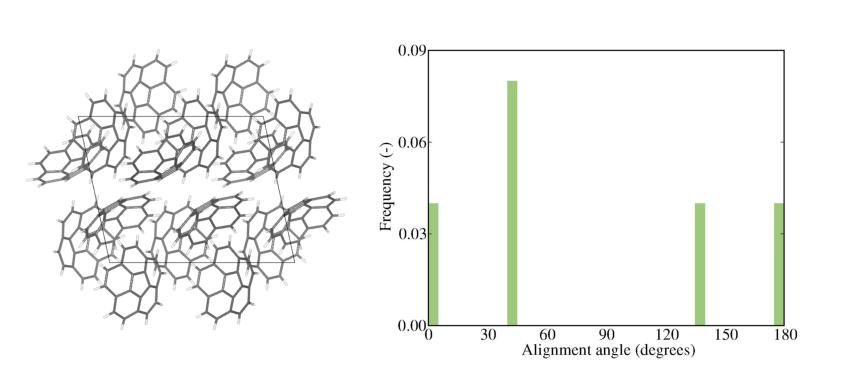
\includegraphics[width=0.65\linewidth]{Figures/corannulene_crystal.eps}
\caption{Snapshot of corannulene crystal structure (left) with alignment angle distribution (right).}
\label{figSI:corannulene_crystal}
\end{figure}
%

\subsection{Cut-off distance sensitivities}
The selection of the cut-off distance, $R$, influences the calculated average intermolecular distances, coordination numbers, and alignment angles.

Due to the molecular arrangements of the homogeneous corannulene clusters (that is, sandwich-type stacking is not present), these results are the most sensitive to the selection of $R$.


Figure \ref{figSI:alignmentangles_cutoffs} shows the alignment angle distributions for all homogeneous clusters using four different cut-off distances.  The influence of the cut-off distance is minimal in the 2pent15ring clusters, which show a very high proportion of molecules with at least one near neighbour at all cut-off distances.  At the higher cut-off distances, a second peak corresponding to further molecule layers (ie not the nearest neighbours alone) appears.  The corannulene clusters show relatively similar angle distributions across the cut-off distances, although the percent of molecules with a near neighbour increases dramatically between $R=0.5$ nm and $R=0.6$ nm.  
%
\begin{figure}[!tbh]
\centering
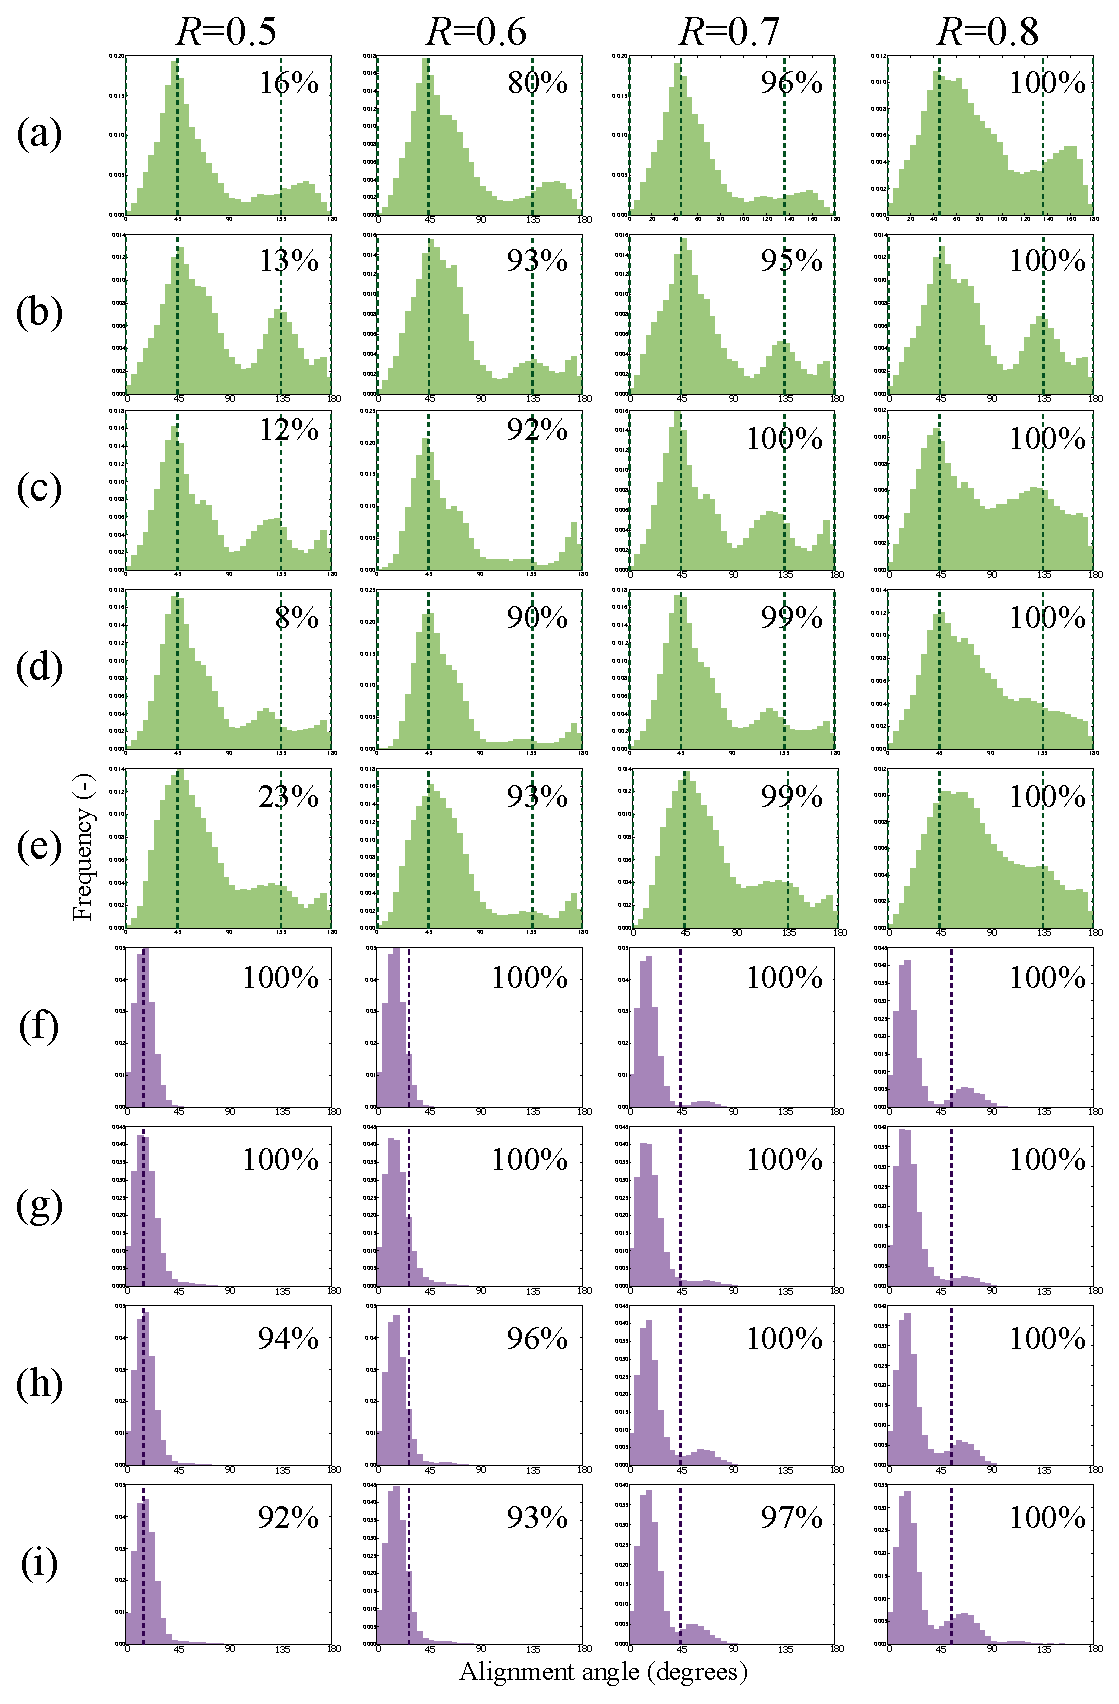
\includegraphics[width=0.85\linewidth]{Figures/AlignmentAnglesCutoffAssessment_SI.eps}
\caption{Alignment angle distributions at different cut-off distances, $R$, in nm for the following clusters: (a) ann\_25, (b) ann\_40, (c) ann\_50, (d) ann\_100, (e) ann\_200, (f) two\_25, (g) two\_40, (h) two\_50, (i) two\_100. Dashed lines correspond to the corannulene crystal structure (for (a)-(e)) and the minimised 2pent15ring dimer (for (f)-(i)). Percent values in the upper right hand corners of each angle distribution refer to the percent of molecules within the cluster that have at least one near neighbour.}
\label{figSI:alignmentangles_cutoffs}
\end{figure}
%

- Include figure of CN histograms with r=0.5 for corannulene and 2pent15ring

Note that for all systems, no neighbouring molecules are found using a cut-off distance of 0.4 nm or smaller.


Table \ref{tableSI:intermolecdistscutoff} presents the average intermolecular distances of homogeneous clusters as a function of the cut-off distance used in analysis. For the corranulene molecule clusters, the cut-off distance selected influences the average intermolecular distance calculated.  Intuitively, an increase in the cut-off distance produces an increase in the average intermolecular distance, since the cut-off distance simply increases the range between 'neighbouring' molecules. At low cut-off values ($r = 0.5$ nm and $r = 0.6$ nm) very few molecule pairs exist and so these averages are not a clear picture of the true average intermolecular spacing throughout the cluster.  At $r = 0.7$ nm, the majority of molecules ($\ge 95$\%) have at least one near neighbour and therefore this provides the best indication of the cluster average.
% perhaps include the % of molecules that have a neighbour in each case?

In contrast, the cut-off distance does not have a large impact on the average intermolecular spacing of homogeneous 2pent15ring molecules.  This highlights the highly stacked configuration of these molecules.




% 
\begin{table}[]
\centering
\caption{Average molecular intermolecular distance, in nm, for homogeneous clusters with varying cut-off values, $r$ in nm, used.}
\label{tableSI:intermolecdistscutoff}
\begin{tabular}{lcccc}
\hline
\multicolumn{1}{l}{\multirow{2}{*}{Cluster}} & \multicolumn{4}{c}{\multirow{1}{*}{Intermolecular distance}} \\
 & $r = 0.5$ & $r = 0.6$ & $r = 0.7$ & $r = 0.8$ \\ \hline
ann\_25 & 0.45 & 0.55 & 0.59 & 0.68 \\
ann\_40 & 0.45 & 0.55 & 0.59 & 0.67 \\
ann\_50 & 0.47 & 0.55 & 0.60 & 0.67 \\
ann\_100 & 0.48 & 0.55 & 0.59 & 0.68 \\
ann\_200 & 0.47 & 0.55 & 0.60 & 0.68 \\ \hline
two\_25 & 0.44 & 0.44 & 0.45 & 0.49 \\
two\_40 & 0.45 & 0.45 & 0.46 & 0.47 \\
two\_50 & 0.45 & 0.45 & 0.48 & 0.50 \\ 
two\_100 & 0.45 & 0.45 & 0.48 & 0.52 \\ \hline
%ann\_40\_Kion\_1 & 0.44 & 0.56 & 0.61 & 0.67 \\
%ann\_40\_Kion\_2 & 0.45 & 0.55 & 0.58 & 0.66 \\
%two\_40\_Kion\_1 & 0.46 & 0.46 & 0.48 & 0.53 \\ \hline
\end{tabular}
\end{table}
%





\subsection{Alignment angles - 100 molecule systems}
%
\begin{figure}[!tbh]
\centering
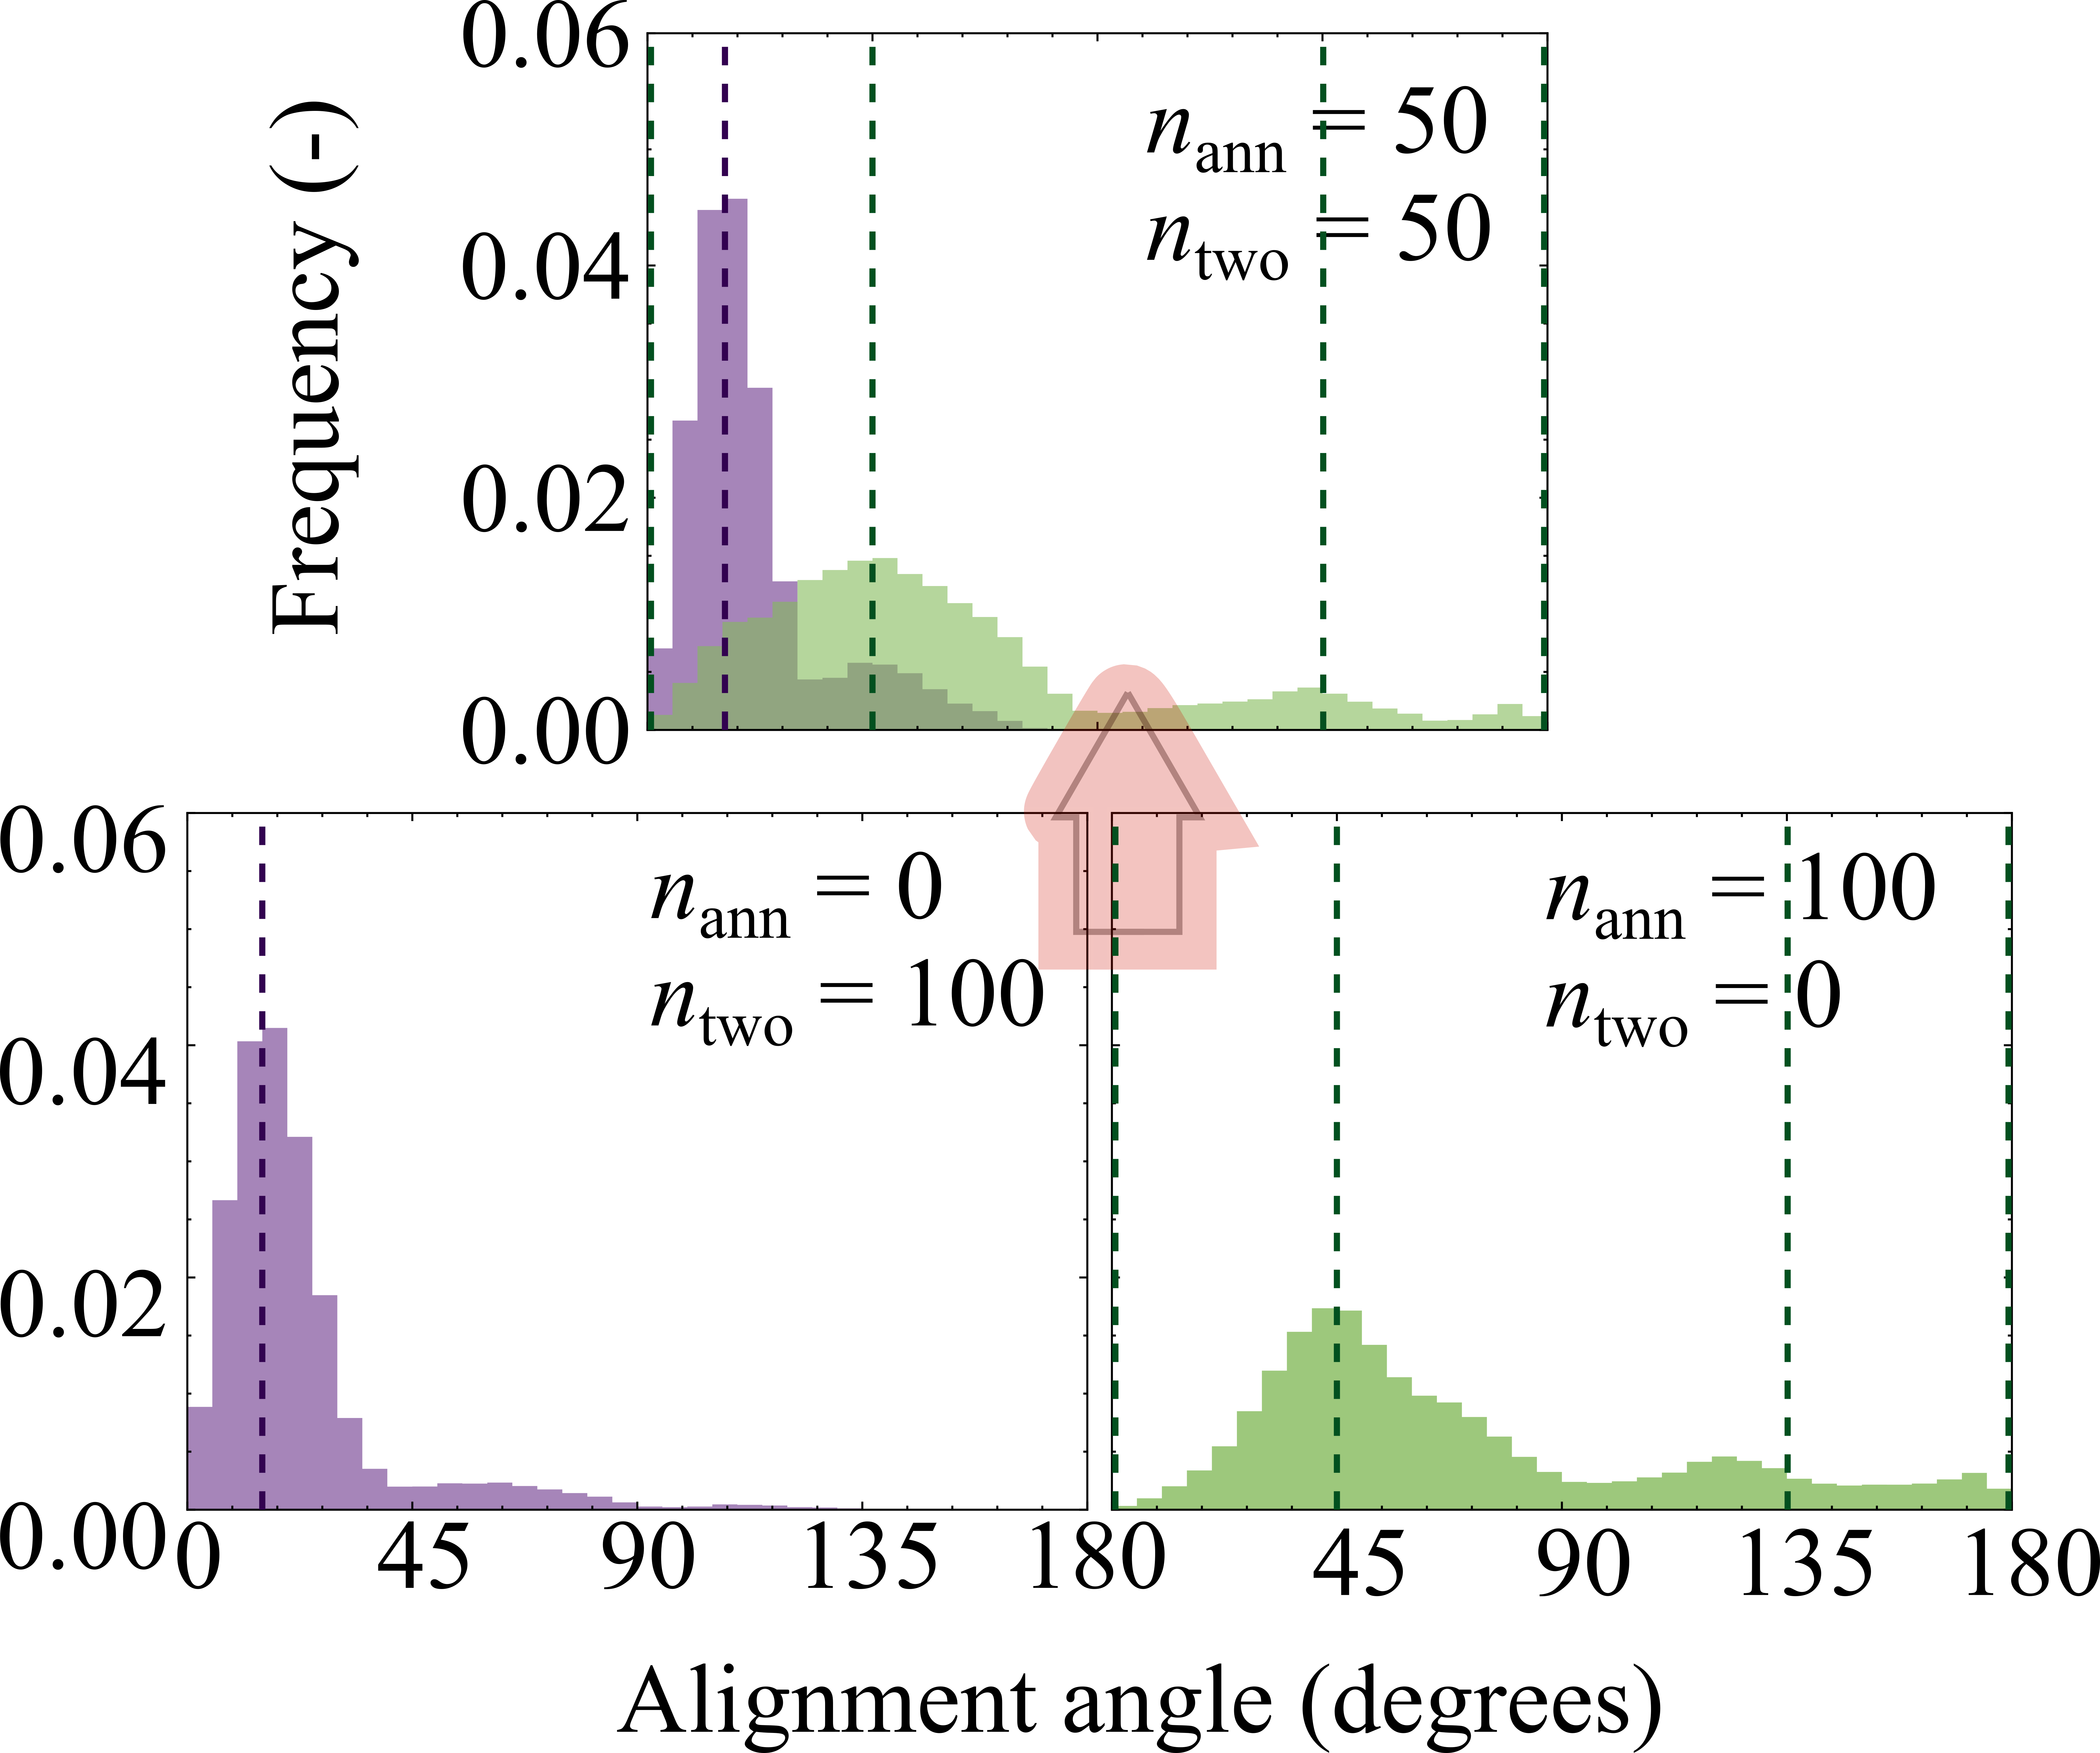
\includegraphics[width=0.5\linewidth]{Figures/alignment_angle_hetero_SI_draft.png}
\caption{Alignment angle distributions for homogeneous and heterogeneous 2pent15ring and corannulene clusters each containing 100 molecules.}
\label{figSI:alignmentangles_100}
\end{figure}
%

\subsection{Radial distances}
Table \ref{tableSI:radialdistances} presents the average equilibrium radial distances for all clusters.  For the homogeneous cases, the two molecule types show similar equilibrium radial distances according to the cluster diameter.  However, in all clusters containing two molecule types the smaller corannulene molecules possess larger radial distances than the larger 2pent15ring molecule.  This is indicative of a core-shell structure in which the larger molecules reside in the cluster core, just as seen in the fPAH clusters \cite{bowal2018partitioning}.

The addition of the potassium cation(s) also result in significant decreases in the radial distances for both molecule types.


%
\begin{table}[]
\centering
\caption{Equilibrium radial distance, in nm, for all clusters studied}
\begin{tabular}{lcc}
\hline
\multicolumn{1}{l}{\multirow{2}{*}{Cluster}} & \multicolumn{2}{c}{Radial distance} \\ 
\multicolumn{1}{c}{} & \multicolumn{1}{c}{corannulene} & \multicolumn{1}{c}{2pent15ring} \\ \hline
ann\_25 & \multicolumn{1}{c}{0.86} & -- \\
ann\_40 & \multicolumn{1}{c}{1.04} & -- \\
ann\_50 & \multicolumn{1}{c}{1.11} & -- \\
ann\_100 & \multicolumn{1}{c}{1.42} & -- \\
ann\_200 & \multicolumn{1}{c}{1.80} & -- \\ \hline
two\_25 & \multicolumn{1}{c}{--} & 1.21 \\
two\_40 & \multicolumn{1}{c}{--} & 1.37 \\
two\_50 & \multicolumn{1}{c}{--} & 1.40 \\
two\_100 & \multicolumn{1}{c}{--} & 1.85 \\ \hline
two\_20\_ann\_20 & \multicolumn{1}{c}{1.28} & 1.14 \\
two\_50\_ann\_50 & \multicolumn{1}{c}{1.83} & 1.50 \\
two\_10\_ann\_30 & \multicolumn{1}{c}{1.18} & 0.96 \\
two\_30\_ann\_10 & \multicolumn{1}{c}{1.50} & 1.25 \\ \hline
two\_40\_K\_1 & \multicolumn{1}{c}{--} & 1.32 \\
ann\_40\_K\_1 & \multicolumn{1}{c}{1.02} & -- \\
ann\_40\_K\_2 & \multicolumn{1}{c}{1.01} & -- \\ \hline
\end{tabular}
\label{tableSI:radialdistances}
\end{table}
%

Figure \ref{figSI:radialdists_molec} shows the average molecular radial distances for molecule types within clusters. Note that the histograms corresponding to the fPAH clusters ((e) and (f)) are smoothed since these results were taken from an REMD simulation instead of a post-REMD MD simulation at a single temperature.
%
\begin{figure}[!tbh]
\centering
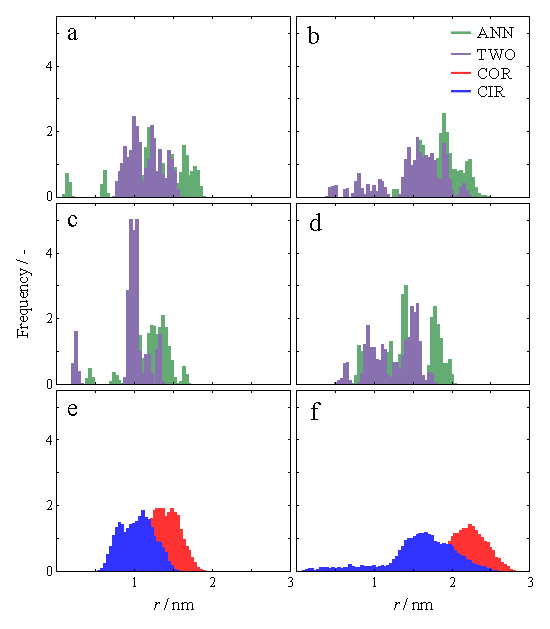
\includegraphics[width=0.5\linewidth]{Figures/molec_histograms.eps}
\caption{Atomic radial distance histograms for (a) two\_20\_ann\_20, (b) two\_50\_ann\_50, (c) two\_10\_ann\_30, (d) two\_30\_ann\_10, and (e) cir\_16\_cor\_16.}
\label{figSI:radialdists_molec}
\end{figure}
%

\newpage